% Homework template for Algorithm Analysis and Design
% UPDATE: September 20, 2019 by Xu Rongchen
\documentclass[a4paper]{article}
\usepackage{ctex}
\ctexset{
proofname = \heiti{证明} %% set proof name
}
\usepackage{amsmath, amssymb, amsthm}
% amsmath: equation*, amssymb: mathbb, amsthm: proof
\usepackage{moreenum}
\usepackage{mathtools}
\usepackage{url}
\usepackage{bm}
\usepackage{enumitem}
\usepackage{graphicx}
\usepackage{subcaption}
\usepackage{booktabs} % toprule
\usepackage[mathcal]{eucal}

\usepackage{iidef} % set homework count
\usepackage{longtable}

% \usepackage[noend]{algpseudocode}
\usepackage{clrscode3e}

\thecoursename{算法分析与设计实验报告}
\theterm{2019年秋季学期}
\hwname{最近点对}
\slname{\heiti{解}}
\begin{document}
\courseheader
\theusername{徐荣琛}
\thestuno{2019214518}
\theinstitute{软件学院}

\info

\begin{enumerate}
  \setlength{\itemsep}{3\parskip}
  %% Homework Start here:
  %% \item to enumerate the problem ID: Format as 'HomeworkID.ProblemID'
  %% \begin{solution} XXXX \end{solution} is to make a solution
  %% \begin{proof} XXXX \end{proof} is to make a proof
  %% Suggest to use \input{path} command
  \textbf{1.实验要求}\\
  实现求平面上最近点对的复杂度为$\Theta(n\lg n)$的算法,要求:\\
  (1)有图形界面,能通过鼠标输入点,并表示出最近点对;\\
  (2)能够随机生产大量平面点(要求可达到一百万个点),并输出最近点对。\\
  并分析比较在不同输入规模情况下$\Theta(n^2)$和$\Theta(n\lg n)$
  算法的实际运行时间。\\  
  \bigskip

  \textbf{2.实验环境}\\
  实验代码采用C\#语言实现,具体的实验环境如下表所示:\\ \medskip
  \begin{tabular}{c|c}
    \hline\hline
    处理器 & Intel(R) Core(TM) i7-8850H CPU @ 2.60GHz \\ \hline
    内存 & 16GB\\ \hline
    操作系统& Mac OS X 10.14.6\\ \hline
    编译环境& .Net Core 3.0.100\\
    \hline\hline
  \end{tabular}\\
  \bigskip

  \textbf{3.实验内容}\\
  \textbf{3.1 复杂度为$\Theta(n\lg n)$的平面最近点对算法实现}\\
  \medskip
  3.1.1 算法实现的具体思路:\\
  (1)将所有点按照y坐标排序(全局仅进行一次,之后保持有序性);\\
  (2)利用线性时间的第k大算法找到有关x坐标中位数对应的点;\\
  (3)根据(2)中得到的点线性时间将所有点分成两部分,此时两部分仍然分别保持(1)中的有序性;\\
  (4)递归两部分的点集合,直到点集合内点个数为1(一个点集合的最近点对距离约定正无穷);\\
  (5)筛选出切割位置左右两侧当前最优解距离内的所有点,对这些点分别计算与上下不超过最优距离的其
  他点的距离,如果优于当前最优解则更新,根据容斥原理,这样的点一定不超过8个,故合并子问题的复杂
  度为线性时间;\\
  \medskip
  3.1.2 算法的优化:\\
  (1)标准的分治法的思路是根据两个子问题的结果的最近距离作为当前最优解再继续进行子问题合并的操作的。
  一个优化在于,设置一个全局的最优解变量,然后所有的距离均和这个全局最优解比较和更新,这样可以利用已知
  信息有效减少其他分支上的问题计算规模,减少算法耗费时间。\\
  \medskip
  \textbf{3.2 支持鼠标输入和结果标识的图形化用户界面的实现}\\
  \medskip
  图形化用户界面使用ASP.Net实现,数据展示采用了开源ECharts可视化图表库,运行时的用户界面输入界面
  如下图所示:
  \bigskip
  \begin{center}
    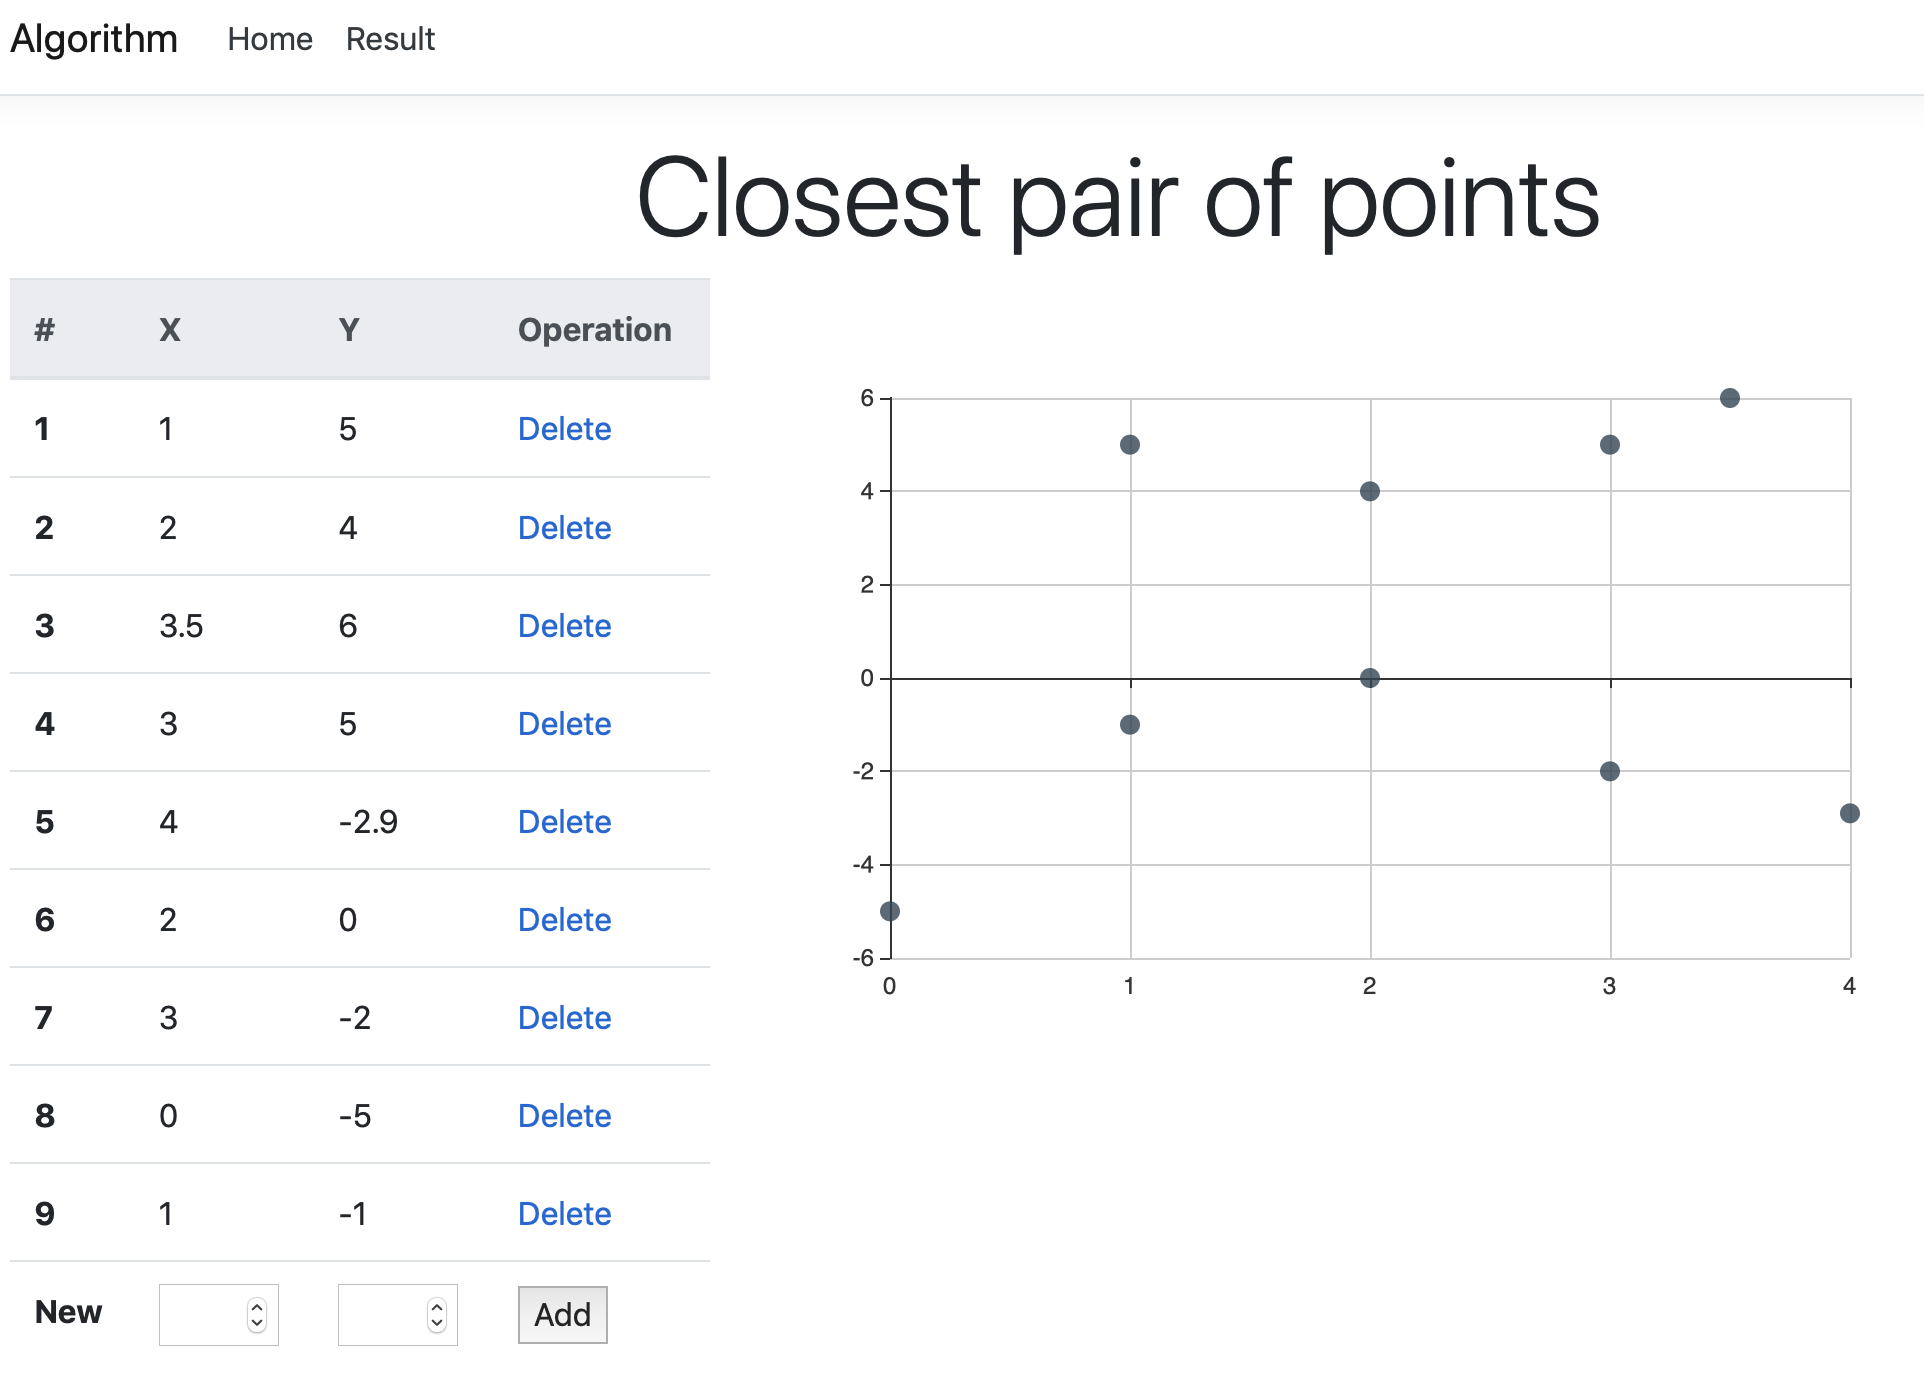
\includegraphics[scale=0.3]{Pictures/cpop1.png}
  \end{center}
  运行后得到最近点对距离和点对的标记如下图所示:
  \bigskip
  \begin{center}
    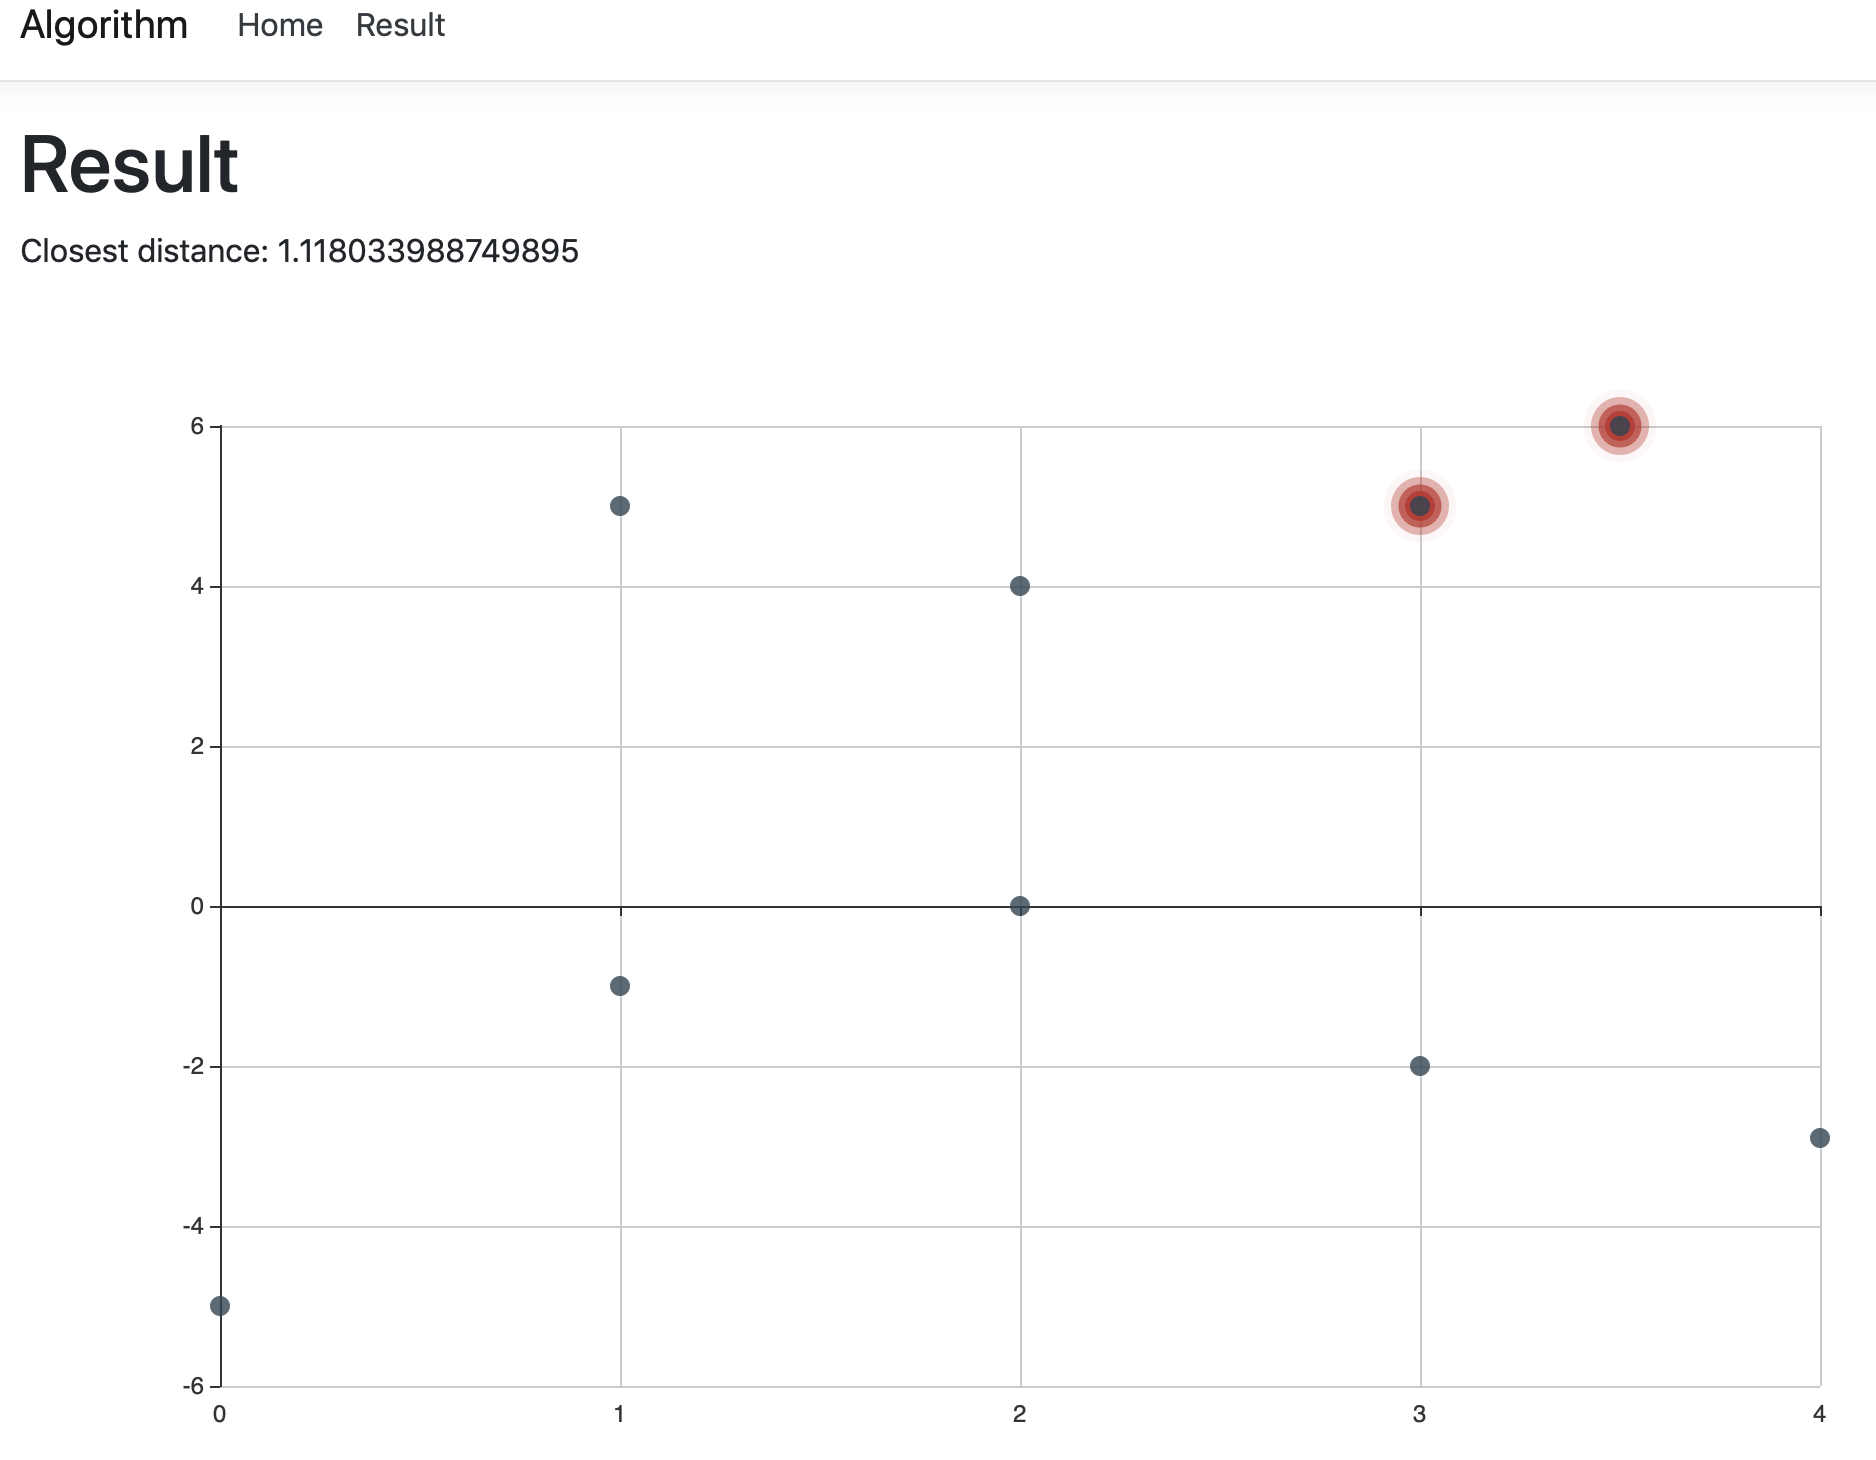
\includegraphics[scale=0.3]{Pictures/cpop2.png}
  \end{center}
  \medskip
  \textbf{3.3 随机一百万个平面点生成并进行求解实验}\\
  \medskip
  随机生成的点人为要求其服从均匀分布,由于点的横纵坐标采用浮点数表示,所以希望得到在某一上下界内均匀
  分布的随即浮点数。.Net Core中$Rand$类提供了$NextDouble()$的方法随机出(0,1)范围内均匀分布的浮点
  数,故采用如下方式得到(LowerBound,UpperBound)范围内均匀分布的浮点数:
  $$NextDouble()*(UpperBound-LowerBound)+LowerBound$$\\
  设定上下界范围为(-100,100),随机1,000,000个点并执行最近点对算法,可以得到以下运行结果:
  \bigskip
  \begin{center}
    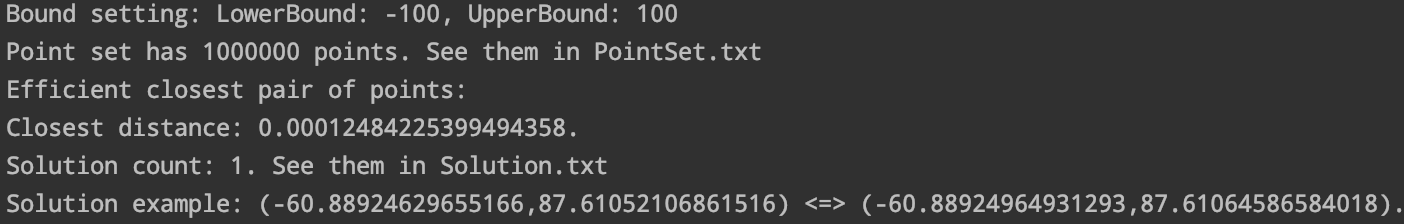
\includegraphics[scale=0.4]{Pictures/log.png}
  \end{center}
  此实验表明算法可以解决一百万个点规模的最近点对问题。\\
  \medskip
  \textbf{3.4 $\Theta(n^2)$和$\Theta(n\lg n)$算法在不同规模随机数据下的对比实验}\\
  \medskip
  3.4.1 实验概要:\\
  对于两种算法,分别随机产生出3组1E2, 5E2, 1E3, 5E3, 1E4, 5E4, 1E5, 5E5, 1E6数据规模的随机点,
  并在这些点集上进行对比实验,设置每组的超时时间为60秒。实验程序编译时设定为Release。\\
  \medskip
  3.4.2 实验结果:\\
  实验结果如下表所示:\\ \medskip
  \resizebox{\linewidth}{!}{ 
  \begin{tabular}{c||ccc|c||ccc|c}
    \hline\hline
    规模& $E1$& $E2$& $E3$& $EA$& $N1$& $N2$& $N3$& $NA$\\ \hline
    1E2&0.00894 &0.00160 &0.00092 &0.00382 &0.00118 &0.00033 &0.00012 &0.00054\\
    5E2&0.00341 &0.00383 &0.00234 &0.00319 &0.00104 &0.00123 &0.00125 &0.00117\\
    1E3&0.00498 &0.00484 &0.00482 &0.00488 &0.00372 &0.00388 &0.00390 &0.00383\\
    5E3&0.01946 &0.02137 &0.02123 &0.02069 &0.06167 &0.06072 &0.05958 &0.06066\\
    1E4&0.04915 &0.04257 &0.04194 &0.04455 &0.19470 &0.18785 &0.19036 &0.19097\\
    5E4&0.20651 &0.21944 &0.22987 &0.21861 &4.23536 &4.23443 &4.49164 &4.32047\\
    1E5&0.63202 &0.41690 &0.40984 &0.48626 &17.51799 &17.18423 &17.14976 &17.28399 \\
    5E5&2.87273 &3.52119 &4.18541 &3.52644 &Timeout &Timeout &Timeout &Timeout\\
    1E6&10.46015 &12.58344 &14.94236 &12.66198  &Timeout &Timeout &Timeout &Timeout\\
    \hline\hline
  \end{tabular}
  }\\
  \medskip
  表中,$E1,E2,E3,N1,N2,N3$分别表示高效算法(Efficient)和暴力算法(Naive)三次实验的结果,$EA,NA$是三次实验的均值。
  时间单位为秒。\\
  \medskip
  3.4.3 实验分析:\\
  以数据规模为横坐标,算法耗时为纵坐标(为方便低数量级的展示,故这里采用对数坐标),绘制出如下的
  耗时曲线比较图:
  \begin{center}
    \includegraphics[scale=0.8]{Pictures/chart.pdf}
  \end{center}
  从图中可发现,当数据规模小于$10^3$数量级时,暴力方法能够更快解决问题,当数据规模超过$10^3$数量级后,
  复杂度为$O(n \lg n)$的算法表现出了明显的计算优势。尤其是,面对5E5和1E6规模的问题时,暴力算法已经不
  能在1分钟内进行求解。\\
  有趣的一点是$O(n \lg n)$的算法在1E2的平均耗时比5E2规模的平均耗时几乎一致(甚至略高),说明数据较小
  时,主要耗时并不由数据规模决定,而是由常数决定。\\
  另一方面,可以发现暴力方法的三次实验用时较$O(n \lg n)$算法更加趋于一致,说明暴力方法时间消耗更加稳定,
  而$O(n \lg n)$算法耗时可能取决于数据内容,这也与算法实现相吻合。
\end{enumerate}


\end{document}